%        File: sheet.tex
%     Created: Mon Mar 14 04:00 PM 2016 C
% Last Change: Mon Mar 14 04:00 PM 2016 C
%
\documentclass[a4paper,twocolumn]{article}

\usepackage{geometry}
\usepackage{amsmath}
\usepackage{amssymb}
\usepackage{graphicx}
\usepackage{float}

\geometry{a4paper, margin={.3in, .3in}}

\title{Computer Vision 1 - Cheat Sheet}
\author{Andrea Jemmett}

\begin{document}
\maketitle

\section{Color Models}
Color is part of the electromagnetic spectrum with energy in the range from 380
to 780 nm wavelength. Most of the colors we perceive are a mixture of
wavelengths where the amount of energy at each wavelength is given by the
spectral energy distribution (SED). When white light shines upon an object, some
wavelengths are absorbed and other are reflected (a green object will reflect
light with wavelength around 500nm, other wavelengths will be absorbed). The
\textbf{hue} corresponds with the dominant wavelength of the SED;
\textbf{saturation} is defined as the proportion of pure light with respect to
white light needed to produce the color; \textbf{lightness} is the intensity of
the reflected light meanwhile \textbf{brightness} is the intensity of the light
source. Let $EH$ be the dominant wavelength in the SED and $EW$ the wavelength
contributing to the white light, then the \textit{hue} is equal to $EH$, the
\textit{saturation} equals to the difference $EH - EW$ and the
\textit{lightness} equals to the area underlined by the SED.

\begin{figure}[htpb]
	\centering
	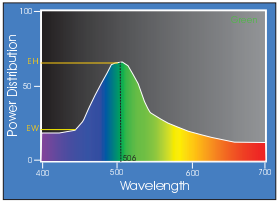
\includegraphics[height=1.5in]{imgs/color-sed.png}
\end{figure}

Experiments have been conducted in which a human observer was asked to adjust
three knobs which control the intensity of a three primary colors so to match
the (perceived) color of the test light. The three primary lights were
additively mixed in and the knobs' values were recorded yielding the so called
color matching functions $\bar{r}(\lambda)$, $\bar{g}(\lambda)$ and
$\bar{b}(\lambda)$. The problem with these was that a negative amount of
at least one of the primaries was necessary to produce the full spectra. So the
CIE proposed a mathematical transformation, the \textbf{XYZ} model, which uses
another set of color matching functions: $\bar{x}(\lambda)$, $\bar{y}(\lambda)$
and $\bar{z}(\lambda)$.

The observer perceives color in terms of three color signals based on the
trichromacy theory and can be modeled as:
\begin{equation} \label{eq:color-perception}
C = \int_{\lambda} E(\lambda) S(\lambda) f_C(\lambda) d\lambda
\end{equation}
where $C \in \{R, G, B\}$, $E$ is the SPD, $S$ is the light reflected by objects
and $f_C$ is the color matching function. If we use $\bar{x}$, $\bar{y}$ and
$\bar{z}$ then we have the XYZ color space. To better represent graphically this
color space we can compute the $xyz$ values as follows:
\begin{equation}
x = \frac{X}{X + Y + Z} \quad y = \frac{Y}{X + Y + Z} \quad z = \frac{Z}{X + Y + Z}
\end{equation}
where we factor out the intensity. Since the chromaticity values sum to unity,
two elements are sufficient to represent a color. When the $x$ and $y$ values
are represented on a plane the chromaticity diagram is obtained. We can also
infer the hue from the chromaticity diagram: first we need to select a reference
white light, the hue is then the wavelength at the spectral curve that
intersects the line from reference light through the color point to the spectral
curve (this point is $G_2$). If $||G_1||$ is the distance from the color to the
white light and $||G_2||$ is the distance from $G_2$ to the white source, then
the saturation is given by $\frac{||G_1||}{||G_2||}$.

RGB values can be obtained using equation \ref{eq:color-perception} and the
$\bar{r}$, $\bar{g}$, and $\bar{b}$ color matching functions. The projection of
RGB points on the rgb chromaticity triangle is defined by:
\begin{equation}
r = \frac{R}{R + G + B} \quad g = \frac{G}{R + G + B} \quad b = \frac{B}{R + G + B}
\end{equation}
In the HSI chromaticity diagram, we compute hue and saturation in the following
way: by assuming white light we define a reference point of $r = g = b = 1/3$,
the saturation can than be computed as:
\begin{equation}
S_{rgb}(r, g, b) = \sqrt{(r - 1/3)^2 + (g - 1/3)^2 + (b - 1/3)^2}
\end{equation}
or
\begin{equation}
S(R, G, B) = 1 - \frac{min(R, G, B)}{R + G + B}
\end{equation}
while the hue is given by:
\begin{equation}
H_{rgb}(r, g, b) = arctan(\frac{r - 1/3}{g - 1/3})
\end{equation}
or
\begin{equation}
H(R, G, B) = arctan(\frac{\sqrt{3}(G - B)}{(R - G) + (R - B)})
\end{equation}

A color invariant system contains color invariant models that are more or less
insensitive to the varying image conditions. For matte surfaces
\textit{RGB} is sensitive to orientation while \textit{rgb} is (assuming
constant white light) insensitive to orientation, illumination direction and
intensity (similarly are S and H). For shiny surfaces H is color invariant.


\section{Surface Reflection}
The Bidirectional Reflectance Distribution Function (BRDF) is the most general
model of light scattering. Describes how much light arriving at an incident
direction $\mathbf{v_i}$ is emitted in a reflected direction $\mathbf{v_r}$. It
can be written as a function of the angles of incident and reflected light like so:
\begin{equation}
f_{BRDF}(\theta_i, \phi_i, \theta_r, \phi_r) =
	\frac{radiance\_of(\theta_r, \phi_r)}{irradiance\_at(\theta_i, \phi_i)}
\end{equation}
Typically BRDF can be split into \textit{diffuse} and \textit{specular}
components. The \textbf{diffuse} component (\textit{Lambertian} or \textit{matte}
reflection) scatters light uniformly in all directions and is associated with
the phenomena of \textit{shading}. Light is scattered uniformly across all
directions (the BRDF is constant):
\begin{equation}
f_d(\theta_i, \phi_i, \theta_r, \phi_r) = \frac{\rho_d}{\pi}
\end{equation}
but the amount of light depends on the angle between the incident direction and
the surface normal $\theta_i$ (is independent of the viewing direction
$\mathbf{v}$):
\begin{equation}
radiance\_of = \frac{\rho_d}{\pi} I cos(\theta_i)
\end{equation}
where $\rho_d$ is the surface albedo and $I$ is the source intensity.
This is because the surface area exposed to a given amount of light becomes
larger at oblique angles. The \textbf{specular} (glossy or highlight) BRDF reflection
depends strongly on the outgoing light direction. All the incident light energy
is reflected in a \textit{single} direction (only when $v_i = v_r$). So the
mirror BRDF is a delta function:
\begin{equation}
f_d(\theta_i, \phi_i, \theta_v, \phi_v) = \rho \delta(\theta_i - \theta_v)
\delta(\phi_i + \pi - \phi_v)
\end{equation}
\begin{equation}
radiance\_of = I f_d(\theta_i, \phi_i, \theta_v, \phi_v)
\end{equation}

Another reflectance model is the \textbf{Phong} model which uses an
\textit{ambient illumination} component besides diffuse and specular.


\section{Image Processing}
We can think of an image as a function from $\mathbb{R}^2$ to $\mathbb{R}$.

\subsection{Point Operators}
Act on a single point, that is locality in the image is lost.
\paragraph{Contrast and Brightness} also called \textit{gain} and
\textit{bias} are defined by the following operation:
\begin{equation}
g(\mathbf{x}) = a f(\mathbf{x}) + b
\end{equation}
where $a$ and $b$ are gain and bias respectively.
\paragraph{Gamma Correction} is used to remove the non-linear mapping between
the input radiance and the pixel values (invert gamma mapping):
\begin{equation}
g(\mathbf{x}) = [f(\mathbf{x})]^{\frac{1}{\gamma}}
\end{equation}
where $\gamma = 2.2$ is a reasonable fit for most cameras.
\paragraph{Histogram Equalization} is used to transform an image so that the
resulting histogram is flat. A pro of this is that we can show the entire color
range, but a flat histogram results in a muddy-looking picture. A solution to
this is to perform a \textit{partial} histogram equalization, that is blend the
full histogram equalization and an identity transform.

\subsection{Neighborhood Processing (Filtering)}
Act on a neighborhood of pixels, that is spatial information is preserved.
\subsubsection{Linear Filters}
This class of filters have the property of being linear (the response to the sum
of two signals is equal to the sum of the responses of the two signals
separately). It could be formulated as follows:
\begin{equation}
g(i, j) = \sum_{k,l} h(k, l) f(i + k, j + l)
\end{equation}
and is called a \textit{correlation}. A common variant is the following:
\begin{equation}
g(i, j) = \sum_{k,l} h(k, l) f(i - k , j - l)
\end{equation}
and is called a \textit{convolution}. Note that a convolution flips the
resulting image because the sign of the offsets has been reversed.

Linear filters suffer from boundary effects, this is because the original image
is being padded with zero valued pixels wherever the convolution kernel extends
beyond the image boundaries. There exist a number of padding techniques:
\textit{zero} sets all pixels outside the image with zeros, \textit{constant}
sets all pixels to a specified border color, \textit{clamp} repeats edge pixels
indefinitely, \textit{cyclic} wraps pixels around the image and \textit{mirror}
reflected pixel along the edge.

\paragraph{Separable filtering}


\end{document}

